\chapter{Lecture 10: Einstein's Equation, Waves, and the Cosmological Constant}

We begin this lecture in a deceptively simple place: empty flat space, then a particle, then the question of what geometry can be flat everywhere except at a point. From there the discussion expands to the physical role of dimension, contracts again to the algebraic form of Einstein's equation, and then turns operational: how do we take an equation we already trust in special relativity and promote it into general relativity? That route leads us to a scalar wave equation in curved spacetime, to a corresponding energy-momentum tensor, and finally back to the cosmological constant, pressure, shear, and asymptotic flatness. These notes follow Leonard Susskind closely, and where a blackboard layout carries part of the argument we keep the LazyingArt LLC and Video2Book evidence nearby rather than replacing it by a cleaner but less faithful memory.

\section{Conical Gravity and a Dimensional Warm-Up}

The lecture opens with a low-dimensional model because it makes curvature visible before it becomes formal. Start with empty spacetime. If there is no energy around, spacetime may be taken to be flat, and a constant-time slice is just an ordinary flat space. Now place a particle into the picture. The right-hand side of Einstein's equation is no longer zero where the particle sits, and we are led to ask for a geometry that is flat everywhere except at one point.

The answer is a cone. In \(2+1\) dimensions, a point mass does not produce the familiar \(1/r\) potential of \(3+1\) gravity. Instead, the spatial geometry is flat away from the source, but with a deficit angle at the location of the mass. The lecture only needs the proportionality,
\begin{equation}
\delta \propto m,
\end{equation}
and does not pause to fix the numerical coefficient.

This point is important: the conical geometry is not restricted to an idealized point particle. If the energy distribution is bounded inside some finite region, then outside that region the geometry is again conical. One may round off the tip, but the exterior remembers only the total deficit.

\begin{figure}
\centering
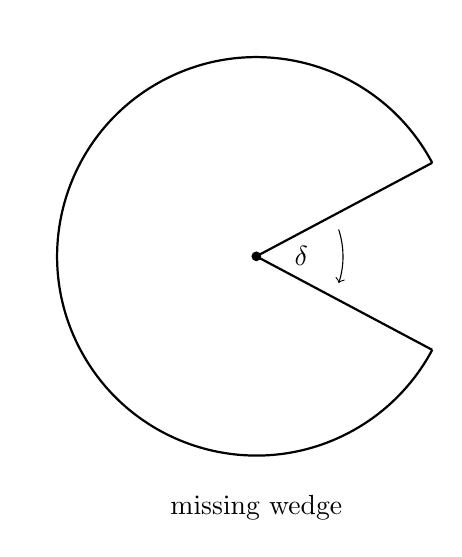
\begin{tikzpicture}[scale=1.1]
\draw[thick] (0,0) -- (28:2.3);
\draw[thick] (0,0) -- (332:2.3);
\draw[thick] (28:2.3) arc[start angle=28,end angle=332,radius=2.3];
\draw[->] (18:1.0) arc[start angle=18,end angle=-18,radius=1.0];
\node at (0.52,0) {\(\delta\)};
\node at (0,-2.9) {missing wedge};
\fill (0,0) circle (1.6pt);
\end{tikzpicture}
\caption{Transcript reconstruction of the conical deficit. Away from the tip the geometry is flat; the source is encoded in the missing angle \(\delta\).}
\end{figure}

From here the lecture makes its first physical payoff. If the deficit angle grows with mass, then one may ask how much mass it takes before the deficit reaches \(360^\circ\). At that point the cone closes up: there is no spatial opening left. The conclusion is qualitative but striking. In \(2+1\) gravity there is only limited room for gravitating matter before space closes on itself. That is why the opening conical picture is not a geometric curiosity. It is already an argument that dimension matters physically.

\section{Why \(3+1\) Matters, and Why Time Counts as a Dimension}

Once the conical example has done its job, the lecture broadens the discussion. Two spatial dimensions are too cramped. One spatial dimension is worse. The physically interesting case is \(3+1\), and the lecture argues this not from pure mathematical necessity but from the behavior of basic physics.

For higher spatial dimensions the force law changes. At the level of this lecture we only need the qualitative comparison:
\begin{equation}
F(r)\sim r^{-2},\qquad r^{-3},\qquad r^{-4},
\end{equation}
as the number of spatial dimensions rises from three to four to five. The exact transcript is garbled in places, but the pedagogical point is clear. In higher dimensions the force becomes more singular at short distance and weaker at long distance, compared with the familiar inverse-square law. Planetary systems become dynamically unstable, and atoms fare even worse: the outer electronic structure is too weakly held while the inner attraction becomes too violent. The lecture's claim is therefore anthropic in the mildest sense: we may not know why nature chose \(3+1\), but we would not be sitting here in a much higher-dimensional world.

\subsection{Question \& Answer}

\paragraph{Question.} Why does time deserve dimensional status at all?

\paragraph{Answer.} The lecture's answer is straight out of special relativity. We call time a dimension because Lorentz transformations mix space and time in the same structural way that ordinary rotations mix spatial directions. There is no unique time axis once different inertial frames are allowed. A moving observer's time direction is tilted relative to ours, and the associated spatial directions tilt with it. This makes it natural to regard spacetime as four-dimensional.

A compact way to say the same thing is that energy and momentum belong to a single four-vector, just as time and space coordinates belong to a single spacetime coordinate system. The signature is not Euclidean; with our convention
\begin{equation}
\eta_{\mu\nu}=\mathrm{diag}(1,-1,-1,-1),
\end{equation}
so time remains distinguished. But distinguished does not mean external to the geometry. It is one coordinate direction in spacetime, and boosts mix it with the spatial ones.

The lecture also fields a question about more than one time dimension and refuses to romanticize it. The answer is simply that such a world is too confusing to think about profitably at this stage. That refusal is part of the rhythm of the lecture: when the physics is clear, pursue it; when it is merely exotic, postpone it.

\section{Einstein's Equation, Covariant Conservation, and the \(\lambda\) Ambiguity}

A student's question about the cosmological constant triggers the first real algebraic spine of the lecture. We want a two-index geometric tensor on the left-hand side, because on the right-hand side sits the two-index energy-momentum tensor \(T_{\mu\nu}\). The simplest geometric candidates are \(R_{\mu\nu}\) and \(g_{\mu\nu}R\). The issue is then to find the correct linear combination.

The lecture arrives at the Einstein tensor
\begin{equation}
G_{\mu\nu}\equiv R_{\mu\nu}-\frac12 g_{\mu\nu}R,
\end{equation}
and emphasizes why the coefficient \(\frac12\) is not ornamental. It is fixed by the requirement of covariant conservation. If \(\nabla_\mu T^{\mu\nu}=0\), then the left-hand side had better satisfy the analogous identity,
\begin{equation}
\nabla_\mu G^{\mu\nu}=0.
\end{equation}
That is the decisive structural fact.

\begin{figure}
\centering

\includegraphics[width=0.62\textwidth]{lecture_10_figure_02.png}
\caption{Covariant conservation and metric compatibility on the board.}
\end{figure}

The lecture then points out that there is one more object with the same covariant-conservation property: the metric itself. In the notation of the board,
\begin{equation}
\nabla_\mu g^{\mu\nu}=0.
\end{equation}
Therefore Einstein's equation is not completely unique. One may add a term proportional to the metric and still preserve covariant conservation:
\begin{equation}
R_{\mu\nu}-\frac12 g_{\mu\nu}R+\lambda g_{\mu\nu}=k\,T_{\mu\nu}.
\end{equation}
This \(\lambda\) is the cosmological constant.

\subsection{Question \& Answer}

\paragraph{Question.} Why may we add \(\lambda g_{\mu\nu}\) without spoiling conservation?

\paragraph{Answer.} Because the covariant derivatives of the metric vanish. The lecture gives the local geometric reason. At any chosen point one may adopt coordinates in which the metric takes the Minkowski form and its first derivatives vanish there,
\begin{equation}
g_{\mu\nu}=\eta_{\mu\nu},\qquad \partial_\alpha g_{\mu\nu}=0
\quad\text{at the point.}
\end{equation}
At that point the Christoffel symbols vanish, so the covariant derivative of the metric vanishes. Since that statement is tensorial, it is true in every coordinate system, not only in the special one chosen at the point.

That is the whole mechanism behind the ambiguity. The Einstein tensor is covariantly conserved, and so is the metric. Therefore the combination \(G_{\mu\nu}+\lambda g_{\mu\nu}\) is covariantly conserved as well.

The lecture immediately adds a physical gloss. The cosmological constant does not behave like an inverse-square correction. In the Newtonian analogy it produces a force proportional to distance. So even before cosmology appears in detail, \(\lambda\) is already telling us that gravity may contain a qualitatively different long-distance piece.

\section{Newtonian Limit and the Status of Einstein's Guess}

A useful correction comes next. The lecture does not want the formal derivation of the left-hand side to sound too triumphant. Einstein's equation is not deduced from pure first principles. It is a tensorial guess, guided by covariance and then checked against Newtonian gravity in the weak, static limit.

Take the \(00\)-component. For slowly moving matter, the dominant component on the right-hand side is the energy density,
\begin{equation}
T_{00}\approx \rho.
\end{equation}
On the left-hand side, once the metric is only weakly perturbed from flat space and the configuration is static, the lecture says that one finds a second spatial derivative of \(g_{00}\). In cautious form,
\begin{equation}
\nabla^2 g_{00}\propto \rho,
\end{equation}
with the warning, explicitly given in the lecture, that the factor of two is easy to confuse.

Now \(g_{00}\) is closely related to the Newtonian potential \(\Phi\). Therefore the weak-field limit becomes the familiar Poisson equation,
\begin{equation}
\nabla^2 \Phi = 4\pi G\,\rho.
\end{equation}
That is the point of contact with Newton. Einstein was looking for a tensor equation which, in the regime of weak fields and slow motions, would reduce to the older theory. It is correspondence, not deduction, and the lecture is careful to preserve that distinction.

This also explains the empirical tone. Once the tensor equation is guessed, it has consequences beyond Newton's theory. When things move fast, or when matter becomes dense enough to generate strong gravitational fields, Newton and Einstein part company. At that point experiment decides, and Einstein wins.

\section{The Equivalence Principle as a Recipe: From Flat-Space Waves to Curved-Space Waves}

Before touching Schwarzschild, the lecture makes a strategic detour. Rather than jumping to exact solutions, it asks how physicists now think operationally about the equivalence principle. The principle is not merely that accelerated frames imitate gravity. The stronger lesson is that in a sufficiently small region, where curvature cannot be detected, the equations of physics should take the special-relativistic form.

This is the modern recipe. If we know an equation in special relativity, we rewrite it as a tensor equation. Then that same tensor equation is taken over into curved spacetime.

The lecture briefly recalls how this works for particles. A free particle moves in a straight line in flat spacetime. General relativity promotes that to the statement that a particle moves along the straightest possible line in curved spacetime: a geodesic. The next example is more instructive because it is field-theoretic rather than mechanical.

Start with a scalar field \(\phi\) in one spatial dimension. The flat-space wave equation is
\begin{equation}
\partial_t^2\phi=c^2\,\partial_x^2\phi.
\end{equation}
In three spatial dimensions we add the other spatial second derivatives,
\begin{equation}
\partial_t^2\phi
=
c^2\left(\partial_x^2+\partial_y^2+\partial_z^2\right)\phi.
\end{equation}
If we now set \(c=1\) and use Minkowski notation, the equation becomes
\begin{equation}
\eta^{\mu\nu}\partial_\mu\partial_\nu\phi=0.
\end{equation}

This is precisely the sort of compact expression the lecture likes: familiar physics compressed into relativistic notation. But then the lecturer deliberately stops at the false summit.

\subsection{Question \& Answer}

\paragraph{Question.} Why is \(g^{\mu\nu}\partial_\mu\partial_\nu\phi=0\) not yet a tensor equation?

\paragraph{Answer.} Because replacing \(\eta^{\mu\nu}\) by \(g^{\mu\nu}\) is only half of the job. The derivative of a scalar, \(\partial_\nu\phi\), is indeed a vector. Raising the index with the metric produces another vector, \(g^{\mu\nu}\partial_\nu\phi\). But once we differentiate that vector, an ordinary derivative is not enough. The derivative of a vector does not transform as a tensor unless we use the covariant derivative.

So the correct curved-space equation is
\begin{equation}
\nabla_\mu\!\left(g^{\mu\nu}\partial_\nu\phi\right)=0.
\end{equation}
Now the equation is genuinely tensorial.

The lecture then uses the Leibniz rule and metric compatibility to clean up the expression. Since covariant derivatives satisfy
\begin{equation}
\nabla_\mu(AB)=(\nabla_\mu A)B+A(\nabla_\mu B),
\end{equation}
we have
\begin{align}
\nabla_\mu\!\left(g^{\mu\nu}\partial_\nu\phi\right)
&=
(\nabla_\mu g^{\mu\nu})\partial_\nu\phi
+
g^{\mu\nu}\nabla_\mu\nabla_\nu\phi \\
&=
g^{\mu\nu}\nabla_\mu\nabla_\nu\phi,
\end{align}
because \(\nabla_\mu g^{\mu\nu}=0\). Therefore the covariant wave equation may be written as
\begin{equation}
\nabla_\mu\nabla^\mu\phi=0.
\end{equation}

The lecture spends time feeling its way through the indices because that is exactly where the conceptual obstacle lies. One must learn not only to replace symbols, but to preserve tensorial meaning. Once this is done, the physical interpretation is immediate. The new equation contains the metric and Christoffel symbols, so the gravitational field appears directly in the propagation law. A wave now moves through a medium whose effective coefficients vary with position. That is why gravity bends waves.

\section{Closing the System: The Scalar-Field Stress-Energy Tensor}

At this point the lecture reverses direction. We have seen how gravity acts on the wave field. Now we ask how the wave field acts back on gravity. In other words: what goes on the right-hand side?

The lecture chooses the simplest setting first: flat spacetime. There the scalar field satisfies
\begin{equation}
\eta^{\mu\nu}\partial_\mu\partial_\nu\phi=0.
\end{equation}
We want a two-index tensor built from \(\phi\). Differentiating \(\phi\) gives indexed objects, so a natural ansatz is
\begin{equation}
T_{\mu\nu}
=
\partial_\mu\phi\,\partial_\nu\phi
+
C\,\eta_{\mu\nu}\,\partial_\sigma\phi\,\partial^\sigma\phi.
\end{equation}
The lecture rejects terms odd in \(\phi\) because energy should not flip sign under \(\phi\to -\phi\). A wave field and the same wave field with opposite sign should have the same energy, just as a harmonic oscillator has the same energy whether the spring is pulled left or right. So the stress tensor must be quadratic.

Now we determine \(C\) by demanding conservation.

\begin{enumerate}
\item Start from the continuity equation
\begin{equation}
\partial^\mu T_{\mu\nu}=0.
\end{equation}

\item Differentiate the first term:
\begin{align}
\partial^\mu\!\left(\partial_\mu\phi\,\partial_\nu\phi\right)
&=
(\partial^\mu\partial_\mu\phi)\partial_\nu\phi
+
(\partial^\mu\phi)(\partial_\mu\partial_\nu\phi).
\end{align}

\item The first piece vanishes because \(\phi\) satisfies the wave equation.

\item Differentiate the second term:
\begin{align}
\partial^\mu\!\left(\eta_{\mu\nu}\,\partial_\sigma\phi\,\partial^\sigma\phi\right)
&=
\partial_\nu\!\left(\partial_\sigma\phi\,\partial^\sigma\phi\right) \\
&=
2\,(\partial^\sigma\phi)(\partial_\nu\partial_\sigma\phi).
\end{align}

\item Since ordinary derivatives commute in flat spacetime, this has the same structure as the remaining term from step 2. Choosing
\begin{equation}
C=-\frac12
\end{equation}
makes the two contributions cancel.
\end{enumerate}

So the stress-energy tensor takes the standard form
\begin{equation}
T_{\mu\nu}
=
\partial_\mu\phi\,\partial_\nu\phi
-
\frac12\eta_{\mu\nu}\,\partial_\alpha\phi\,\partial^\alpha\phi.
\end{equation}
This is the same expression that appears on the board.

\begin{figure}
\centering

\includegraphics[width=0.86\textwidth]{lecture_10_figure_03.png}
\caption{Scalar-field stress-energy tensor and the \(T_{00}\) energy density.}
\end{figure}

The lecture then asks for the energy density. With our signature, \(T_{00}\) is
\begin{align}
T_{00}
&=
\dot{\phi}^{\,2}
-
\frac12\left[
\dot{\phi}^{\,2}
-
\left(\frac{\partial\phi}{\partial x}\right)^2
-
\left(\frac{\partial\phi}{\partial y}\right)^2
-
\left(\frac{\partial\phi}{\partial z}\right)^2
\right] \\
&=
\frac12\left[
\dot{\phi}^{\,2}
+
\left(\frac{\partial\phi}{\partial x}\right)^2
+
\left(\frac{\partial\phi}{\partial y}\right)^2
+
\left(\frac{\partial\phi}{\partial z}\right)^2
\right].
\end{align}
That is exactly the combination the lecture wants us to recognize: kinetic energy plus gradient energy. The violin-string analogy is not decoration. It tells us how to read the formula. The \(\dot{\phi}^{\,2}\) term is kinetic. The spatial derivative terms are the elastic energy stored in the field configuration.

There remains one overall normalization ambiguity, but the lecture treats it correctly as conventional. One may rescale \(\phi\) and absorb any overall multiplicative factor into the field definition. So once the relative coefficient is fixed, the tensor is essentially unique.

\section{Pressure, Localized Sources, and the Cosmological Constant Revisited}

Having constructed one explicit \(T_{\mu\nu}\), the lecture broadens the meaning of source. Gravity does not respond only to rest mass or even only to energy density. Pressure and shear are also present in the energy-momentum tensor, and therefore also gravitate.

In an isotropic situation the off-diagonal spatial components vanish and the diagonal spatial entries may be identified with pressure. If the system is not isotropic, one must think more generally in terms of stresses. Off-diagonal components represent shear. The lecture even remarks that a shear stress can be reinterpreted as unequal diagonal stresses after a \(45^\circ\) rotation. So Einstein's source is not merely mass density in disguise; it is the full local bookkeeping of energy, momentum, and stress.

\subsection{Question \& Answer}

\paragraph{Question.} If the source is localized, why is the field not zero elsewhere?

\paragraph{Answer.} Because the field equation is local, but its solutions are not compactly supported just because the source is. The lecture returns to the Newtonian analogy:
\begin{equation}
\nabla^2\Phi = 4\pi G\,\rho.
\end{equation}
If \(\rho\) vanishes outside the material source, that does not force \(\Phi\) to vanish there. It only tells us that the appropriate combination of derivatives vanishes there. Solving the equation still produces a nontrivial exterior field, the familiar \(1/r\) potential and \(1/r^2\) force.

The same logic applies in general relativity. \(T_{\mu\nu}\) may vanish outside the matter distribution, yet the metric and curvature need not be trivial there. The exterior geometry is determined by matching to the source and by solving the field equations in the surrounding vacuum region.

The lecture then takes up a related question: if light carries energy and momentum, can light gravitate against light? In principle yes. One may estimate the interaction schematically as
\begin{equation}
F \sim G\,\frac{E_1E_2}{c^4\,r^2}.
\end{equation}
The structure is the important part. Because the effective masses are \(E/c^2\), the interaction is suppressed by powers of \(c\), and with Newton's constant already tiny the effect is negligible in ordinary laboratory conditions. So gravitational self-interaction of light does not visibly spoil the superposition principle for everyday beams, even though the principle is not exact in the full nonlinear theory.

The lecture also remarks qualitatively that black holes support an unstable circular null orbit. That is a preview, not a result to be developed here. The exact geometry is being saved for Schwarzschild.

\subsection{Question \& Answer}

\paragraph{Question.} Why does the cosmological constant not stabilize Einstein's static universe?

\paragraph{Answer.} First recall the Newtonianized picture of \(\lambda\). Up to the sign convention, a uniform cosmological term behaves like a uniform source spread through space. A function with constant Laplacian is
\begin{equation}
\Phi_\Lambda(\mathbf{x})
=
\frac{\lambda}{6}\left(x^2+y^2+z^2\right),
\end{equation}
so that
\begin{equation}
\nabla^2\Phi_\Lambda=\lambda.
\end{equation}
Differentiating gives
\begin{equation}
\frac{\partial \Phi_\Lambda}{\partial x}=\frac{\lambda}{3}x,
\qquad
\frac{\partial \Phi_\Lambda}{\partial y}=\frac{\lambda}{3}y,
\qquad
\frac{\partial \Phi_\Lambda}{\partial z}=\frac{\lambda}{3}z.
\end{equation}
Thus the force is proportional to distance, not inverse square. Depending on the sign, it is either repulsive or attractive. The lecture emphasizes that such a force law does not single out a privileged center. If everything is pushed away from everything else, every observer sees the same kind of recession.

This already explains why the cosmological constant may be interpreted in two ways. One may leave it on the geometric side,
\begin{equation}
R_{\mu\nu}-\frac12 g_{\mu\nu}R+\lambda g_{\mu\nu}=k\,T_{\mu\nu},
\end{equation}
or move it to the right and think of it as a vacuum contribution to stress-energy,
\begin{equation}
R_{\mu\nu}-\frac12 g_{\mu\nu}R
=
k\,T_{\mu\nu}-\lambda g_{\mu\nu}.
\end{equation}
The lecture says, half jokingly, that \(\lambda\) is schizophrenic about which side of the equation it wants to live on. Physically, both readings are useful.

Einstein's historical mistake was subtler. He tried to balance ordinary gravitational attraction against a repulsive cosmological term in order to hold the universe static. But the balance point is unstable. The lecture explains this with an ordinary mechanical picture: one combines the attractive Newtonian potential with the potential associated with a repulsive force proportional to distance. The resulting effective potential has a stationary point, but it is a maximum, not a minimum.

\begin{figure}
\centering
\begin{tikzpicture}[scale=1.0]
\draw[->] (-0.2,0) -- (5.5,0) node[right] {$r$};
\draw[->] (0,-3.1) -- (0,1.4) node[above] {$V(r)$};
\draw[thick] plot[smooth] coordinates {(0.8,-2.8) (1.1,-1.9) (1.6,-1.1) (2.3,-0.35) (3.0,0.18) (3.8,-0.15) (4.8,-1.5)};
\fill (3.0,0.18) circle (1.8pt);
\node[above] at (3.0,0.18) {unstable equilibrium};
\end{tikzpicture}
\caption{Transcript reconstruction of Einstein's static-universe balance. The tuned point is a maximum of the effective potential, so any small displacement sends the system away from equilibrium.}
\end{figure}

That is why the static universe fails. A delicate cancellation may exist, but it does not create a stable resting point. A small perturbation makes the system run away.

Finally, the lecture separates asymptotic flatness from cosmological geometry. If the mass distribution is localized and \(\lambda=0\), then the metric can approach Minkowski space far away:
\begin{equation}
g_{\mu\nu}\to \eta_{\mu\nu}
\qquad\text{as } r\to\infty.
\end{equation}
That is what asymptotically flat means.

With a cosmological constant, the far geometry is different. In vacuum we have
\begin{equation}
R_{\mu\nu}-\frac12 g_{\mu\nu}R+\lambda g_{\mu\nu}=0.
\end{equation}
Contracting with \(g^{\mu\nu}\) in four dimensions yields
\begin{equation}
R-2R+4\lambda=0
\qquad\Longrightarrow\qquad
R=4\lambda,
\end{equation}
with the warning that the lecture itself treats the overall sign of \(\lambda\) loosely at this point. The invariant statement is that a nonzero cosmological constant gives a nonzero uniform curvature even in empty spacetime. The geometry at infinity is then de Sitter or anti-de Sitter, not flat Minkowski space.

\section{Summary}

The lecture begins with a cone and ends by clearing the ground for Schwarzschild. In between, it establishes four durable ideas. First, dimension is physically consequential: low-dimensional gravity and high-dimensional force laws both go wrong in characteristic ways. Second, Einstein's equation is selected by covariance, by conservation, and then by the Newtonian limit, but it still contains the \(\lambda g_{\mu\nu}\) ambiguity. Third, the equivalence principle works as a recipe: rewrite flat-space laws as tensor equations and then carry them into curved spacetime. Fourth, the source of gravity is the full energy-momentum tensor, including pressure and shear, not merely rest mass.

The next step is now clear. We have the field equation, we have learned how matter and waves enter it, and we have seen what sorts of geometrical behavior to expect at infinity. The natural target is the first exact solution of real interest: the Schwarzschild metric.